%% Modified documentstyle to documentclass -- compatibility with LaTex2e
%% N. Mancell (98/03/01).

%%  ucalgthes_root.tex        (NM 98/03/01)
%   Modified   92-09-18      Add references to dissertation        D. Teale
%                            Add approval page to toc
%                            Add ref to Title Degree on approval page
%   Modified  2006-09-12     Added geometry package to set up UofC thesis margins
%                            Removed includeprompt option N. Mancell               
%
\documentclass{ucalgthes1}   
\usepackage[letterpaper,top=1in, bottom=1.22in, left=1.40in, right=0.850in]{geometry}
\usepackage{fancyhdr}
\fancyhead{}
\fancyfoot{}
\renewcommand{\headrulewidth}{0pt}
\fancyhead[RO,LE]{\thepage}  
%Define other usepackages here
\usepackage[plainpages=false]{hyperref}
\title{Auto-tagging Emails and Instant Messages with User Stories to Build a Knowledge Base\\ 
\bigskip for Distributed Agile Projects}
%
%            Insert the correct information between the {}
%
\author{S. M. Sohan}
\thesisyear{2010}
\thesis{thesis}    % the word dissertation can be inserted between {}
\newcommand{\thesistitle}{Auto-tagging Emails and Instant Messages with User Stories to Build a Knowledge Base for Distributed Agile Projects}
\monthname{December}
\dept{COMPUTER SCIENCE}
\degree{MASTER OF SCIENCE}
%
%                    End of supplied information
%
\begin{document}
\makethesistitle
\pagenumbering{roman}     % resets page counter to one
\setcounter{page}{1}
\chapter*{UNIVERSITY OF CALGARY \\ FACULTY OF GRADUATE STUDIES}
\thispagestyle{empty}
The undersigned certify that they have read, and recommend
to the Faculty of Graduate Studies for acceptance, a \Thesis\ entitled
``\thesistitle'' submitted by \Author\
in partial fulfillment of the requirements for the degree of
\Degree.\\

%
%                 Substitute  List of Examiners
%
\begin{signing}{Department of Academic Computing}
\signline
Supervisor, Dr. Frank Oliver Maurer \\
Department of Computer Science \\

\signline
Chairman, Dr.~John D.~Doe \\
Department of Academic Computing \\
Services  \\
\signline
Chairman, Dr.~John D.~Doe \\
Department of Academic Computing \\
Services  \\
\signline
Chairman, Dr.~John D.~Doe \\
Department of Academic Computing \\
Services  \\
\end{signing}
%
\newpage
\phantomsection
\altchapter{Abstract} 
Paragraph 1

Paragraph 2

Paragragh 3
\newpage
\phantomsection
\altchapter{Acknowledgements}
I have been blessed with the trust and support of a number of people and organizations while working on this research. In this regard, I would like to thank -

Dr. Frank Maurer and Dr. Michael Richter for your help with formulating and advancing this research. You have provided me with useful guidelines and suggestions at various steps and kept trust in me all the way.

Syed Rayhan and the Code71 team for providing me with an excellent environment for learning and innovative thinking. Working with you have been a memorable experience and helped me coming up with this research idea.

University of Calgary for your financial support without which I couldn't carry out this research.

My loving wife Shahana for giving me a happy family life. You have come all the way from Dhaka to Calgary to accompany me and that proved to be a lot for my well being.

My parents, S. M. Afaz Uddin and Mrs. Kh. Shirin, for inspiring me all through my life. Your continuous inspiration has given me the enthusiasm and courage at all walks of the life and this graduate research is one example of that.

Bangladesh, my country, for your promise to educate and raise me. You have given me the strong foundation to face the world.

\begin{singlespace}
\newpage
\phantomsection
\tableofcontents
\pagestyle{plain}
\newpage
\phantomsection
\listoftables
\pagestyle{plain}
\newpage
\phantomsection
\listoffigures
\pagestyle{plain}
\clearpage
\end{singlespace}
\clearpage          % otherwise tables will be numbered wrong

\pagenumbering{arabic}
\fancyhead[RO,LE]{\thepage}
\fancyfoot{} 
\chapter{INTRODUCTION}
Agile software engineering process is a collaborative approach to incrementally deliver software in small iterations (e.g. two to four weeks). Agile teams commonly use ``user stories'', a small description of a desired feature in everyday language, to capture the requirements. An example user story is as follows:\\
\emph{As a shopper, I want to pay online to checkout my shopping cart using MasterCard, Visa or Amex credit card from a secured web page only.}\\

The details of such user stories are discussed as an ongoing basis among the people involved in a project. For example, as the engineering team start working on the stories, they often consult with customers and other teammates to further clarify such user stories. Whenever possible, face-to-face communication is preferred as the principal communication medium between customers and developers in agile processes \cite{am} \cite{xp} \cite{scrum} \cite{xp_up}. In collocated setups, where the people work in close proximity, such informal communication relays the tacit knowledge among the people. 

However, for distributed projects, especially when there is a huge time zone difference among people, face-to-face communication become infeasible. As a result, people use alternatives to mitigate this shortcoming such as phone calls, emails, instant messaging, wiki, web forums and so on. So, in such setups communication is often text based instead of tacit knowledge sharing. In this sense, distribution makes it easy to capture the knowledge since much of it is textual and electronic. For an example, considering the aforementioned user story, the developer may send the following email to the customer to further clarify expectations.\\
\emph{\textbf{Subject:} Clarification required on online credit card payment\\
\textbf{Hi Bob:}\\
Please clarify if the shoppers need to provide the security code of the credit card while doing checkout.}

Since email is a persistent tool, one can use this knowledge in future. But, email is also a personal tool and its hard to transfer a selection of project related emails from the rest in a reusable format. So, when someone leaves the team, it becomes hard to access that knowledge when needed later down the road. To retain these useful knowledge, this thesis implemented and evaluated a tool called ``Taggy'' that automatically grabs and tags the emails and instant messages with relevant user stories.

The relationship between a user story and email or instant message is not explicit. To establish the implicit relation, Taggy uses a machine learning technique, Case Based Reasoning (CBR). The CBR system looks at the text, people and temporal similarity between emails and user stories. The evaluation results show that a well trained software can auto-tag emails with user stories. Also, we found that combining context information with text similarity helps to find the related user stories with higher accuracy than using just text match alone.

In the existing literature attempts have been made to capture software project related knowledge following several alternative approaches. For example, commercial tools exist that link software code commit messages with a requirement or ticket given the ticket number is present inside the commit log. Also, another approach is to use wiki or online message threads, where the contents are manually linked with the user stories. However, to use such approaches, one needs to remember identifiable tokens or learn markup syntax (e.g. wiki), which is often burdensome for business users. To reduce this learning curve and human efforts, Taggy builds a knowledge base by automatically tagging emails and instant messages with user stories. 

The remaining part of this chapter is organized as follows: First, I discuss the necessary background material about user story and distributed agile projects to develop a shared understanding of the terms used in this thesis. Then, the research motivation is discussed. Finally, I present the research goals and related challenges.

%Start the body text
\section{User Stories - An Overview}
In agile projects, user stories are used to capture requirements. In short, user stories represent the need for a feature from the view point of a potential user of a software. Mike Cohn\cite{user_stories_applied} defines user stories as follows:\\
A user story describes functionality that will be valuable to either a user or purchaser of a system or software. User stories are composed of three aspects:
\begin{itemize}
	\item a written description of the story used for planning and as a reminder
	\item conversations about the story that serve to flesh out the details of the story
	\item tests that convey and document details that can be used to determine when a story is complete
\end{itemize}

As outlined in the above definition, conversation plays a central role in fleshing out the details of the user stories. Ron Jeffries \cite{ron_jeffries} and Rachel Davies\cite{rachel_davies} also emphasize the role of conversation being a key component of user stories.

Another popular acronym INVEST suggested by Bill Wake \cite{bill_wake} that defines good stories being Independent, Negotiable, Valuable to users, Estimable, Small and Testable. However, to hold all these characteristics yet being Small essentially points to conversation as means of detailing the user stories.

In an agile project, the customer or a representative of the customer is responsible for coming up with these user stories with the help of the stakeholders. Next, the user stories are prioritized in a list known as ``Product Backlog''. At every iteration (typically two to four weeks), the team picks the top user stories from the product backlog known as ``Iteration Backlog'' with the target to deliver the user stories at the end of the iteration. A user story is supposed to be limited to a scope so that it can be delivered within the iteration. However, the details about the user stories are laid out as on going basis during the iteration through customer collaboration and feedback.

One or more team members are assigned to deliver a user story, which may involve design, development, testing and such tasks. It is a common practice that the customer and the assigned people collaborate to fine tune the user story details.

\section{Distributed Agile Projects}
The members of a distributed agile project work from different geographical locations and adopt agile principles. In practice, the distribution can take several models such as the following three outlined by Braithwaite et al \cite{xp_expanded}:

\begin{enumerate}
	\item Agile outsourcing - the development team is offshore to the customer.
	\item Agile dispersed development - developers spread over different locations, such as open source projects.
	\item Distributed agile development - customers are distributed and one development team is distributed evenly to stay close to the customers.
\end{enumerate}

Again, the geographical distribution can be anywhere between offices across the road to opposite part of the world. For example, a team may work for a customer at the same city or a country separated by ten hours of time zone difference. Distributed agile teams often use different electronic communication channels such as Emails, Instant Messaging, Wiki and Forums as well as online project management tools to uncover the important details about the user stories.

Cost has been identified as one of the principal deciding factors for distributing projects across the globe \cite{practical_considerations}. However, projects also go distributed to utilize global talent supply and local knowledge \cite{required}. Previous studies have reported success with distributed agile projects. For example, Sutherland et al. reported a linear scalability with a globally distributed outsourced team following a Fully Distributed Scrum (Scrum is a popular agile method) model \cite{fully_distributed}. Similarly, Yahoo! had success with distributed teams that valued people over process and exercised the right information sharing formats and timing \cite{yahoo}.

To ensure a shared view of the ``Product Backlog'' and ``Iteration Backlog'' distributed teams often use web based project management tools. There are a number of such tools available commercially as well as open-source \cite{required}. Such tools help people working remotely to have a single backlog and collaborate around that. 

\section{Research Motivation}
The existing literature about collaboration in distributed agile software projects suggest the use of various electronic mediums to counter for missing face-to-face communication. Because of time zone difference, such teams often use asynchronous communication tools such as email, wiki in addition to synchronous ones such as telephone call, instant messaging etc. For example, Robarts \cite{practical_considerations} found that teams would follow up with a written email after they had a telephone meeting to ensure the message is clearly understood. Moreover, of all the available written communication tools, email has been regarded as the most-widely used one by several former studies \cite{collab_in_distributed} \cite{on_coord}. Additionally, even in collocate settings, people often use emails to communicate as it doesn't require immediate response and overheads like scheduling meetings.

Although having multiple communication channels adds flexibility for collaboration, it also means the knowledge gets fragmented across different channels. This fragmented knowledge may be spread over the project management tool, wiki, emails, instant messages and other places. To retain the important details about the user stories, one needs to combine these fragmented pieces. But looking into email inboxes of colleagues may be difficult, if not impossible. Even worse, when a teammate leaves, the emails are gone as well. So, the fragmented pieces of knowledge is either lost or very hard to combine together. Even if one has access to the emails, manually copy-pasting all the emails and combining with the relevant user stories would be a time consuming task to say the least. The following user story and email collaboration shows an example of the knowledge fragmentation:

\textbf{User Story (Available in Project Management Tool)}\\
\textbf{Title:} ``As a/an VM System I want to load Auction data from NADA data file''\\
\textbf{Description:} Please see the 3 documents related to Auction data
\begin{enumerate}
\item Auc Layout
\item \textbf{Regions Table}
\item AucData.zip
\end{enumerate}

In this example, the user story represents a data integration with a company named NADA. NADA provides vehicle auction information for regions denoted by a ``region code''. However, as the developer starts working on NADA integration, she asks the following question about the region code to the customer through email. 

\textbf{Email\#1 (From Developer to Customer)}\\
\textbf{Subject:} ``Initial Questions regarding NADA region value''\\
\textbf{Body:} We found that the Region value can be \textbf{Alpha-numeric} that will be received from NADA Auction. But, the NADA WS accepts only \textbf{Numeric} Region value. Is there any conversion rule to convert the region value into numeric? \\
Thanks

To answer this question, the customer replies with the following email.

\textbf{Email\#2 (From Customer to Developer)}\\
\textbf{Subject:} ``RE: Initial Questions regarding NADA region value''\\
\textbf{Body:} I talked to NADA and they provided me with the \textbf{attached conversion table} for \textbf{Alpha-numeric} to \textbf{Numeric} region codes.

Please note that the email from the customer included a conversion table for ``region codes''. 

Given this example, if a person only looks at the user story, she will find partial information about it. So, the whole conversion of ``region code''  may be confusing to her. However, when she can see the emails along with the user story, she may have a better understanding about this user story.

This information may be required since a distributed agile team have to cope up with changes in team composition as new people will join and some people may leave. So, if it is possible to combine the fragmented knowledge from different places such as emails, instant messages and project management tools, one can find the important details of the user stories. Such details many not be obvious when only the user story is available. Similarly, the knowledge can help in testing of the features since it is expected to contain customer feedbacks and clarifications on user stories.

The motivation for this thesis stems from the pursuit of developing a knowledge base by combining the fragmented knowledge from emails, instant messages and project management tools with the least possible human efforts.

\section{Research Problem}
In software development projects, developers sometimes leave the team for various reasons. As said before, in distributed agile projects, important knowledge is often shared by emails. To transfer this knowledge for future use, one first needs to find the project related emails. Secondly, such setups people often use web based project management tools to capture user stories and planning information. If the emails can be related to specific user stories in the project management tools, then another developer of the team will be able to easily find the necessary information about a user story when required.

From an end users' point of view, manually finding and relating the emails with user stories is a time-consuming and costly process. This essentially means copying the emails from inbox and putting into a system and linking with a user story. This manual process is cumbersome to say the least. However, if a software can do this, then it may work as a knowledge-base even after someone leaves the team. Such a software needs to be unobtrusive for the most part so that it doesn't require much human effort. So, a technical solution needs to be in place that can capture the project related communication without violating people's privacy. For example, it cannot look into the email inbox of a developer nor should ask a developer to manually enter the chat log into the system.  

The core technical challenge in devising such a software solution is understanding the emails and relating them to specific user stories. The relation between an email and a user story is not explicit. Alternative approaches to make it explicit, such as using identifiable tokens in email subjects, also makes the communication process obtrusive as it adds an extra step to lookup the identity or memorizing it before writing an email. To alleviate this extra step, one can modify email clients to do the lookup. But doing so for the multitude of emails clients including the ones on mobile phones is cumbersome. Also, it imposes a behavioral change or a learning curve for the for the people at the business end.

To find out the implicit relation between a free-format email and a use story, a software needs to handle similarity between two texts, which is a standard problem. Emails may not show very high text similarity with the related user stories. This text component makes the relevance between a user story and an email an approximation or fuzzy match. Also, pure text retrieval limits how accurate the assignment of email and user stories can be. This is because people use different vocabulary and often a tacit communication is there underneath a written form. Using context information has the potential to increase this accuracy. So, a software needs to be able to combine both the text and context similarity for auto-tagging emails with user stories.

To account for the context, one needs to use the associated meta information that are available. The contexts of an email and a user story are not exactly similar. For example, the context of an email has a time-stamp, sender, recipients and past conversations. On the other hand, user stories have a different context, such as their development time or iteration timeframe, developers and customers. An auto-tagging solution needs to use these context meaningfully so that each component gets its deserving share of importance in the relevance computation. So, it is important to have a formula that produces similarity ranking considering the fuzzy text similarity and associated context relevance.

Next technical challenge is to evaluate the accuracy of the auto-tagging system. For the auto-tagging to be useful, it shouldn't make too many mistakes in finding similarity. The accuracy of this system needs to be tested using real world data. 

Another technical challenge is to design an adaptive auto-tagging system so that it can adapt to different communication patterns. Since distributed agile teams across the world have differences in who, how and when they communicate about their user stories, the auto-tagging system needs to adjust its similarity computation accordingly. For example, one team might spend more time communicating about user stories that are currently under development while another team might prefer to discuss about the upcoming ones. An auto-tagging system that uses the meta information of time needs to learn this pattern to make a right decision.


\section{Research Goals}
The principal goal of this research is to develop a tool that can automatically read and relate emails with user stories based on agile project context. The tool needs to minimize human efforts in doing so. Another complementary goal is to evaluate the tool using real world data. The underlying approach and evaluation of Taggy is discussed in Chapter X.

This research also aimed to investigate the difficulties in solving the various aspects of the research problem, namely i) relevance ranking of user stories for a given email, ii) using text similarity in addition to context relevance, iii) evaluating auto-tagging accuracy and iv) developing an adaptive auto-tagger. The findings from this investigation is expected to provide a foundation for next level of research in this area.

\section{Key Contributions}
This research work has been published and presented at XP 2010 \cite{auto_tagging}. 

The key contribution of this research is, it demonstrates a novel approach of building a knowledge-base for distributed agile teams from emails and user stories. This approach has the similar motivation as found in some previous works, such as clustering emails archives\cite{required}, tagging forum messages with source code change set\cite{required} and using wiki to share knowledge. However, this research shows a machine learning approach to conglomerate fragmented knowledge from emails, instant messages and project management tools minimizing human efforts. This new technique adds to the existing body of knowledge.
                                  
Another key contribution is, it shows that text and context similarity can be used to find relevance between two different types of entities such as emails and user stories, where the degree of text similarity may be inadequate. We have used Case Based Reasoning (CBR) for auto-tagging. As this research findings suggest, other CBR systems concerning different entities may utilize this technique.
\fancyhead[RO,LE]{\thepage}
\fancyfoot{} 
\chapter{RELATED WORK}
Researchers have attempted to solve the problem of knowledge management for software development projects from different point of views. Also, the industry is using a number of available commercial and open-source tools to retain and manage knowledge. To find the similarity and contrast of this research with the existing approaches, this related work chapter is divided into sections dedicated to the following five areas:

\begin{enumerate}
	\item Communication in distributed teams
	\item Wiki based knowledge sharing
	\item Online forum based knowledge sharing
	\item Mining email archives
	\item Exiting tool support for knowledge sharing
\end{enumerate}

\section{Communication in Distributed Teams}
The Agile Manifesto\cite{agile_manifesto} puts heavy emphasis on customer collaboration. Understandably in distributed projects, the geographical and temporal distance accounts for communication challenges compared to a collocated setup. Several existing research focused on the use and effectiveness of the different communication channels that are used in distributed projects.

Thissen et al. points out that a distributed team to become successful must use appropriate tools to ensure easy flow of information \cite{communication_tools}.

%\include{chapter3}
%\include{chapter4}
%\include{chapter5}
% \appendix
% %!TEX root = /Users/smsohan/Taggy/Thesis/ucalgthes1_root_0.tex
\fancyhead[RO,LE]{\thepage}
\fancyfoot{} 
\chapter{Ethics Approval}

The ethics approval for conducting the qualitative evaluation of Taggy is given at Figure~\ref{fig:ethics}:

\begin{figure*}[bt]
	\centering
	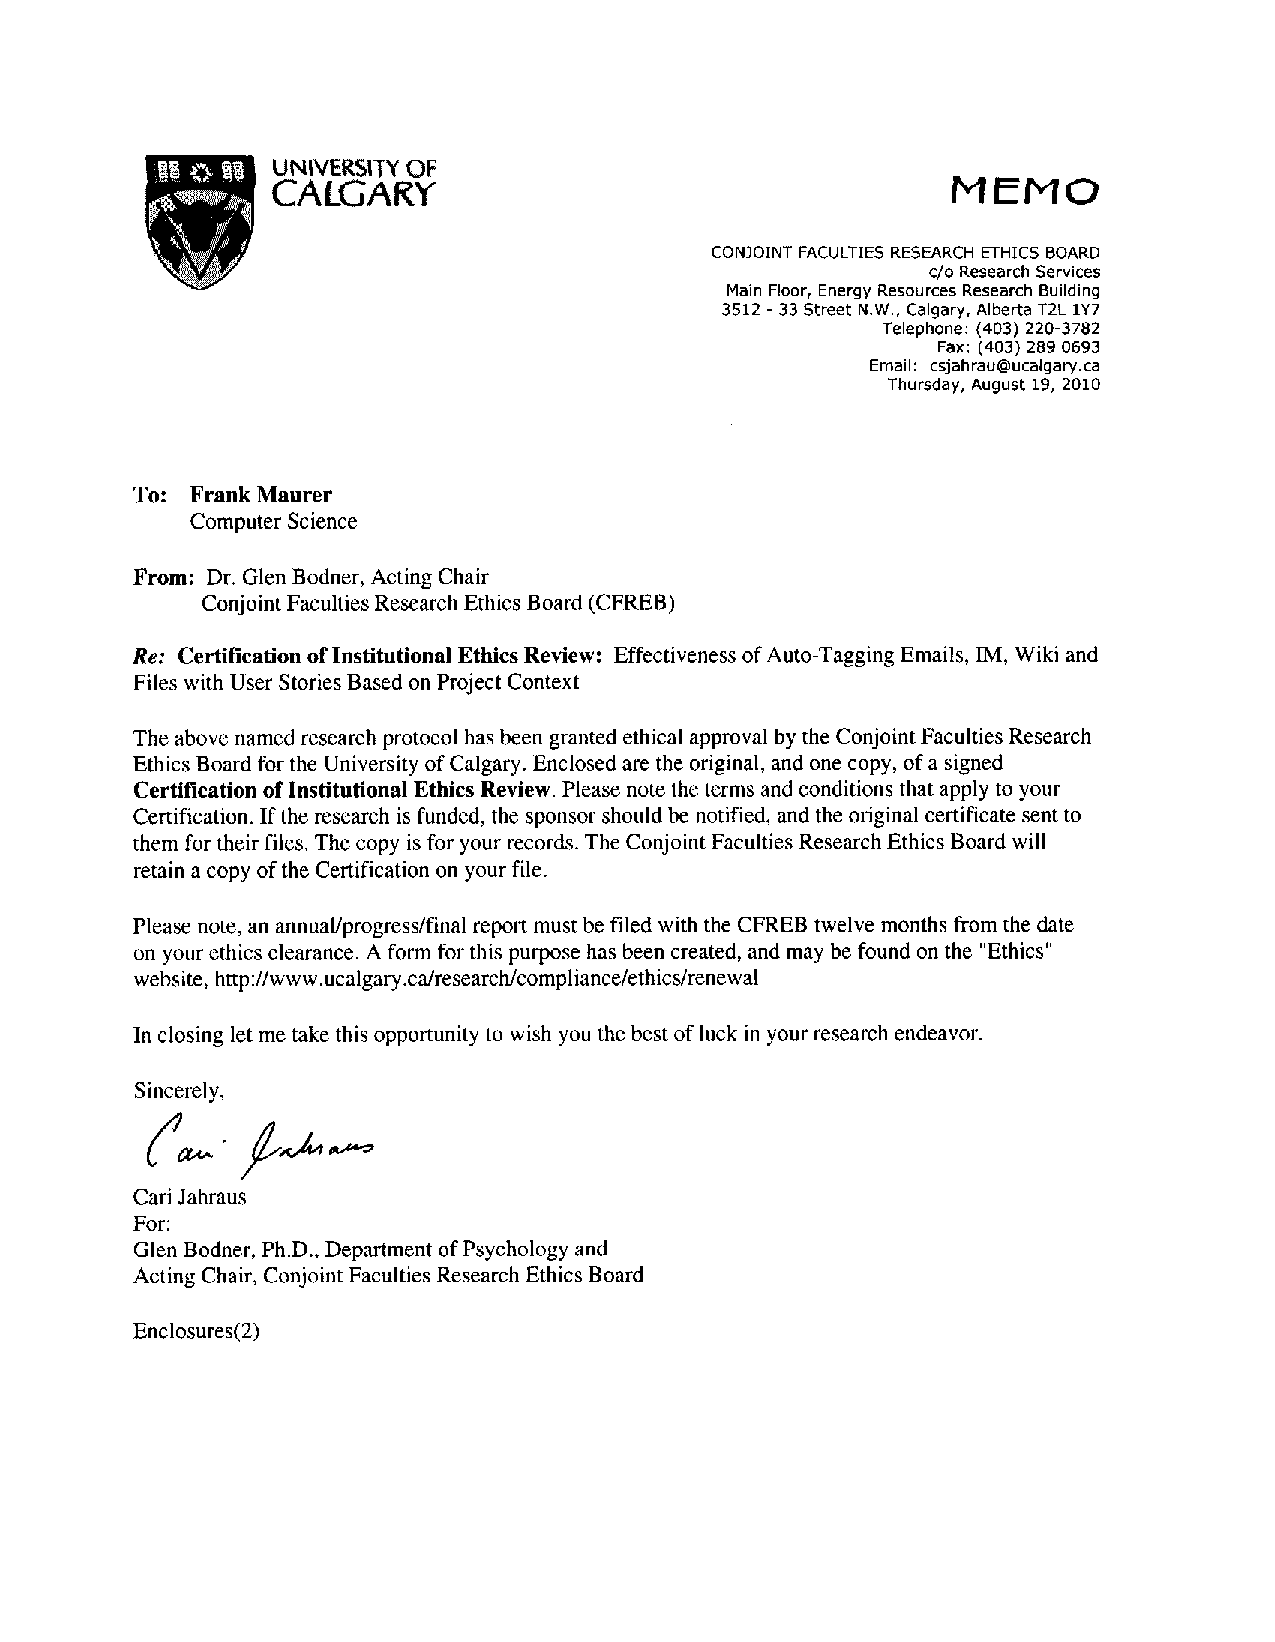
\includegraphics[width=\textwidth]{ethics.pdf}
    \caption{Ethics Approval}
	\label{fig:ethics}
\end{figure*}




\end{document}
